\documentclass[12pt]{article}

% UTF-8 encoding and fonts
\usepackage[utf8]{inputenc}
\usepackage[T1]{fontenc}
\usepackage{lmodern}

% Page setup
\usepackage[margin=1in]{geometry}
\usepackage{setspace}
\onehalfspacing

% Typography
\usepackage{microtype}

% Math and symbols
\usepackage{amsmath,amssymb}

% Graphics
\usepackage{graphicx}
\usepackage{float}
\usepackage{subcaption}

% Tables
\usepackage{booktabs}
\usepackage{array}
\usepackage{multirow}
\usepackage{threeparttable}
\usepackage{longtable}
\usepackage{pdflscape}
\usepackage{siunitx}
\sisetup{detect-all=true, group-separator={,}, group-minimum-digits=4}

% Bibliography
\usepackage{natbib}
\bibliographystyle{aer}

% Hyperlinks
\usepackage{hyperref}
\hypersetup{
    colorlinks=true,
    linkcolor=blue,
    citecolor=blue,
    urlcolor=blue
}
\usepackage[nameinlink,noabbrev]{cleveref}

% Timing data
\IfFileExists{timing_data.tex}{\input{timing_data.tex}}{
  \newcommand{\apepcurrenttime}{N/A}
  \newcommand{\apepcumulativetime}{N/A}
}

% Captions
\usepackage{caption}
\captionsetup{font=small,labelfont=bf}

% Section formatting
\usepackage{titlesec}
\titleformat{\section}{\large\bfseries}{\thesection.}{0.5em}{}
\titleformat{\subsection}{\normalsize\bfseries}{\thesubsection}{0.5em}{}

% Custom commands
\newcommand{\E}{\mathbb{E}}
\newcommand{\Var}{\text{Var}}
\newcommand{\Cov}{\text{Cov}}
\newcommand{\ind}{\mathbb{I}}
\newcommand{\sym}[1]{\ifmmode^{#1}\else\(^{#1}\)\fi}

% Figure notes environment
\newenvironment{figurenotes}{\par\medskip\small\noindent\textit{Notes:} }{\par}

\title{Does Welfare Simplification Encourage Entrepreneurship?\\Evidence from Universal Credit}
\author{APEP Autonomous Research\thanks{Autonomous Policy Evaluation Project. Correspondence: scl@econ.uzh.ch} \and @olafdrw}
\date{\today}

\begin{document}

\maketitle

\begin{abstract}
\noindent
Can simplifying welfare systems encourage firm creation? I study the United Kingdom's Universal Credit reform, which consolidated six legacy benefits into a single payment. Exploiting the staggered rollout across 332 Local Authorities between 2015 and 2018, I estimate the reform's effect on new company registrations using Companies House administrative data and the \citet{callaway2021difference} estimator. I find a precise zero: the point estimate is 0.005 additional firms per 1,000 population per month (95\% CI: $[-0.032, 0.042]$), ruling out increases larger than 16 percent of the mean formation rate. Results are consistent across three modern staggered DiD estimators. An exploratory test of the Minimum Income Floor yields imprecise results. Despite removing a labyrinth of six overlapping programs, the most comprehensive welfare simplification in British history did not measurably increase formal business creation.
\end{abstract}

\vspace{1em}
\noindent\textbf{JEL Codes:} J68, H53, L26, I38 \\
\noindent\textbf{Keywords:} Universal Credit, welfare reform, entrepreneurship, firm formation, difference-in-differences

\newpage

\section{Introduction}

In 2012, a self-employed person in the United Kingdom claiming welfare navigated a labyrinth: six different benefits, three administrative systems, and effective marginal tax rates that could exceed 90 percent. For a benefit claimant considering starting a business, the system's complexity was itself a barrier---not just to claiming support, but to entering self-employment in the first place. A growing body of evidence documents how benefit design affects employment margins \citep{chetty2008moral, krueger2002labor}, yet one dimension has received almost no attention: \textit{complexity}. When navigating multiple overlapping benefits requires substantial effort and expertise, the system may inadvertently discourage the very activities it means to support---particularly self-employment, where income fluctuates and interacts with multiple benefit streams simultaneously.

The United Kingdom's Universal Credit (UC) reform offers an unusually clean test of whether welfare simplification affects entrepreneurship. Introduced between 2015 and 2018, UC replaced six separate means-tested benefits---Jobseeker's Allowance, Employment and Support Allowance, Income Support, Housing Benefit, Working Tax Credit, and Child Tax Credit---with a single monthly payment governed by a unified 55 percent taper rate. For self-employed claimants, the reform also introduced two consequential features: real-time earnings verification through HMRC integration, and the Minimum Income Floor (MIF), which assumes self-employed claimants earn at least the national minimum wage after a twelve-month start-up period. The net effect on entrepreneurship is theoretically ambiguous. Simplification reduces the informational and administrative barriers to becoming self-employed, but the MIF creates a binding floor that penalizes low earners---precisely the group most likely to be marginal entrepreneurs.

I exploit the staggered rollout of UC's ``full service''---the complete digital version available to all claimant types---across more than 300 Local Authorities (LAs) in Great Britain between November 2015 and December 2018. The Department for Work and Pensions (DWP) implemented the rollout in monthly waves, with some LAs gaining access years before others. I construct a novel dataset linking the official DWP rollout schedule to administrative data from Companies House---which records every new company registration in England, Wales, and Scotland with exact incorporation dates and postcodes---and to ONS population estimates for rate normalization.

Using the \citet{callaway2021difference} estimator for staggered difference-in-differences, which is robust to heterogeneous treatment effects across cohorts, I estimate the causal effect of UC full service on firm formation rates. The identification relies on comparing changes in firm creation across LAs that adopted UC at different times, with not-yet-treated LAs serving as the comparison group. I find that Universal Credit had no detectable effect on company registrations. The point estimate is a near-zero 0.005 additional firms per 1,000 population per month. More importantly, the results are precise enough to rule out any increase larger than 16 percent of the mean formation rate---a striking null for the most ambitious welfare simplification in British history.

This paper contributes to the literature on welfare reform and entrepreneurship in three ways. First, I provide the first causal estimate of how welfare simplification affects entrepreneurship, using an identification strategy that credibly isolates the reform's effect. The existing literature on UC focuses on employment transitions \citep{dwp2024employment} and mental health \citep{brewer2024universal}; the self-employment margin has been studied only qualitatively \citep{griffiths2024going}. The null result is itself informative: it bounds the magnitude of welfare complexity as a barrier to firm creation and suggests that other frictions---capital access, risk, human capital---may dominate.

Second, I conduct an exploratory test of the Minimum Income Floor's behavioral effects. The MIF's twelve-month start-up grace period creates a change in incentives facing new self-employed UC claimants, and I test whether the aggregate formation effect attenuates after twelve months, when the MIF begins to bind. This test is necessarily imprecise---the twelve-month threshold applies to individual claimants, not to LAs, so the LA-level split is an ecological proxy---but it speaks to an ongoing policy debate about whether the MIF deters viable businesses \citep{griffiths2024going}.

Third, I provide sector-level heterogeneity that illuminates the mechanism. If UC's effect operates through the self-employment simplification channel, it should be concentrated in sectors with high self-employment propensity---construction, professional services, and transport---rather than sectors like public administration or utilities where self-employment is rare. I test this prediction and use public administration as a placebo.

The results contribute to several literatures. Most directly, this paper speaks to the welfare-and-work literature, which has traditionally focused on the employment-unemployment margin \citep{moffitt2002welfare, blundell2006earned}. The self-employment margin is quantitatively important---the UK has approximately 4.2 million self-employed workers, representing 13 percent of total employment \citep{ons2019selfemployment}---but its interaction with benefit design is poorly understood. The paper also contributes to the entrepreneurship literature, which has documented how access to capital \citep{hurst2004liquidity}, health insurance \citep{fairlie2011entrepreneurship}, and unemployment insurance \citep{hombert2020can} affect business creation, but has not examined how the \textit{administrative complexity} of the safety net shapes entry decisions. Finally, the paper speaks to the broader literature on program complexity as a policy instrument \citep{bhargava2015psychological, finkelstein2019take}, extending it from take-up decisions to labor market transitions.

The remainder of the paper proceeds as follows. Section~\ref{sec:background} describes the UC reform and its implications for self-employment. Section~\ref{sec:data} presents the data sources and panel construction. Section~\ref{sec:empirical} describes the empirical strategy. Section~\ref{sec:results} presents the main results, heterogeneity analysis, and MIF timing test. Section~\ref{sec:robustness} contains robustness checks and sensitivity analyses. Section~\ref{sec:discussion} discusses the interpretation and limitations of the findings. Section~\ref{sec:conclusion} concludes.


\section{Institutional Background}
\label{sec:background}

\subsection{The Legacy Benefit System}

Before Universal Credit, the UK's working-age safety net comprised six separate means-tested benefits, each with its own application process, assessment criteria, reporting requirements, and taper rates. A self-employed individual receiving Housing Benefit, Working Tax Credit, and Child Tax Credit would simultaneously navigate three different administrative systems, each with different rules about how business income affected entitlement.

This complexity created three specific barriers to self-employment. First, \textit{informational barriers}: understanding how self-employment income would interact with multiple benefits required expertise that most claimants lacked. The \citet{uk2013uc} noted that the legacy system's complexity ``created confusion and uncertainty, discouraging claimants from taking up work.'' The six benefits operated on different assessment periods---some weekly, others monthly, still others annual---and used inconsistent definitions of income. A claimant considering starting a small business would struggle to predict how fluctuating earnings would affect each benefit stream.

Second, \textit{administrative barriers}: changes in self-employment income triggered recalculations in multiple systems, often with significant delays, creating cash-flow uncertainty. Housing Benefit assessments, for instance, could take weeks to adjust after an income change, during which the claimant faced either overpayments (requiring future repayment) or underpayments (creating financial hardship). This unpredictability was particularly damaging for self-employment, where income naturally varies from month to month.

Third, \textit{marginal tax rate discontinuities}: the interaction of multiple taper rates could create effective marginal tax rates exceeding 90 percent at certain income levels \citep{mirrlees2011tax}, making it difficult for claimants to predict the return to additional effort. A self-employed person earning slightly above a threshold might lose more in benefit reductions than they gained in additional income---a ``poverty trap'' that the legacy system's fragmented design made nearly impossible for claimants to navigate rationally.

The scale of the potentially affected population was substantial. In 2015, approximately 2.5 million working-age individuals claimed one or more of the six legacy benefits that UC would replace. Of these, survey evidence suggests that roughly 15--20 percent expressed interest in self-employment but cited benefit complexity as a barrier \citep{griffiths2024going}. Even if only a fraction of these individuals were marginal enough to be affected by simplification, the potential for a measurable effect on firm formation existed.

\subsection{Universal Credit Reform}

UC replaced the six legacy benefits with a single monthly payment, calculated using a unified 55 percent taper rate on net earnings above a work allowance. The reform fundamentally changed how the benefit system interacted with self-employment through three key features.

\textit{Simplified reporting.} UC integrates with HMRC's Real Time Information (RTI) system, which automatically reports earnings from employment. Self-employed claimants report earnings monthly through the UC online portal, rather than navigating multiple reporting systems. This single reporting channel replaces the previously fragmented system where different benefits required different forms, submitted to different agencies, on different schedules. The cognitive and administrative burden of benefit management is substantially reduced.

\textit{The start-up period.} New self-employed claimants receive a twelve-month ``start-up period'' during which their UC entitlement is calculated based on actual reported earnings, even if these are very low or zero. This feature effectively provides a subsidy to entrepreneurial experimentation: a claimant can attempt self-employment while retaining full UC entitlement during the crucial early phase when most businesses generate minimal income. Under the legacy system, there was no equivalent provision---starting a business could immediately trigger benefit reductions across multiple programs.

\textit{The Minimum Income Floor (MIF).} After the start-up period, UC calculates entitlement as if self-employed claimants earn at least the national minimum wage multiplied by their expected hours (typically 35 hours per week). If actual earnings fall below this floor, the claimant receives less UC than they would under actual earnings. The MIF was designed to prevent long-term benefit dependency disguised as self-employment, but critics argue it penalizes viable businesses in their early stages \citep{griffiths2024going, uk2018selfemployment}. The House of Commons Work and Pensions Committee heard testimony from multiple self-employed UC claimants who reported that the MIF had forced them to abandon viable businesses because early-stage income fell below the floor \citep{uk2018selfemployment}.

The theoretical prediction is ambiguous. The simplification channel---reduced informational barriers, unified taper rate, single reporting system---should increase self-employment entry on the margin. But the MIF channel works in the opposite direction, creating a new barrier that did not exist under the legacy system. The net effect depends on the relative magnitudes: whether the simplification gains in the first twelve months dominate the MIF-induced deterrence that follows. This is precisely what the MIF timing test is designed to decompose.

\subsection{The Staggered Rollout}

The UC full service---the complete digital version covering all claimant types---was rolled out across Great Britain's Jobcentre Plus offices in monthly waves between November 2015 and December 2018. The DWP selected the rollout order based primarily on IT infrastructure readiness and Jobcentre capacity, not on local labor market conditions \citep{dwp2018rollout}. This is a crucial institutional feature for identification: the as-good-as-random assignment of treatment timing allows for a credible difference-in-differences design.

The rollout proceeded in distinct phases. The first areas---London Borough of Croydon and Southwark---went live in November 2015 as part of an initial pilot. A handful of additional areas joined through 2016, but the pace was slow as the DWP monitored the system's performance. The rollout accelerated dramatically in 2017, with dozens of areas transitioning each month. Most areas had completed the transition by December 2018, though some LAs experienced delays beyond the original schedule. The rollout experienced two ``firebreak'' periods---August-September 2016 and August-September 2017---during which no new areas were added, creating natural breaks in the treatment timing that contribute identifying variation. In the analysis, I classify the 43 LAs whose full service transition was not completed by December 2018 as ``never-treated'' during my study window (January 2013 to December 2019). Most of these LAs transitioned in 2019, making them more precisely ``late-treated'' rather than permanently untreated. For this reason, the preferred Callaway-Sant'Anna specification uses \textit{not-yet-treated} LAs as the comparison group rather than relying exclusively on the never-treated designation. The not-yet-treated comparison pool is larger and does not require that the 43 LAs be permanently untreated---only that they have not yet been treated at the time of comparison.

Figure~\ref{fig:rollout} displays the rollout timeline, showing both the number of LAs transitioning in each month and the cumulative adoption curve. The S-shaped adoption pattern---slow initial adoption, rapid acceleration in 2017--2018, and final completion---is characteristic of IT-driven infrastructure rollouts and reinforces the plausibility of the DWP's stated rationale for the ordering.

\begin{figure}[t]
\centering

\includegraphics[width=\textwidth]{figures/fig1_rollout_timeline.pdf}
\caption{Universal Credit Full Service Rollout Timeline}
\label{fig:rollout}
\begin{figurenotes}
The figure shows the number of Local Authorities transitioning to UC full service in each month (bars) and the cumulative number of LAs with full service (line). The rollout spanned November 2015 to December 2018, with acceleration in 2017--2018. ``Firebreak'' pauses in August-September 2016 and 2017 are visible as gaps. Source: DWP Transition Rollout Schedule (2018).
\end{figurenotes}
\end{figure}

Between 2015 and 2018, observationally similar LAs had different exposure to UC simply because of where they fell in the rollout queue. This staggered adoption creates the identifying variation for the empirical strategy. With 27 distinct treatment cohorts (monthly adoption dates) and 43 never-treated LAs, the design offers substantial variation in both treatment timing and comparison group composition.

An important distinction exists between UC ``full service'' and earlier ``live service'' deployment. Live service, available from 2013 in some areas, covered only single, unemployed claimants making new claims---a small fraction of the target population. Full service extended UC to all claimant types, including self-employed individuals, couples, and those with housing costs. I use the full service date as the treatment, since this is when the self-employment-relevant features (simplified reporting, start-up period, MIF) became available to the population that could plausibly respond on the entrepreneurship margin.


\section{Data}
\label{sec:data}

\subsection{Companies House Registrations}

The primary outcome is new company registrations from Companies House, the UK's official registrar of companies. Companies House maintains a public register of every company incorporated in England, Wales, and Scotland. I use the BasicCompanyData bulk download, which contains the current register of companies with their incorporation dates, registered addresses, SIC codes, and company types. Because this snapshot captures companies on the register as of the download date, companies that were incorporated during the study period but subsequently dissolved before the download are not included. I discuss this survivorship issue and why it does not threaten identification in Section~\ref{sec:discussion}.

I construct monthly formation counts by LA as follows. First, I filter to companies incorporated between January 2013 and December 2019, yielding a study window that encompasses the full pre-treatment period (2013--2015), the rollout period (2015--2018), and a post-rollout period (2018--2019) while avoiding COVID-era confounding that would complicate identification from 2020 onward. This window produces approximately 1.46 million company registrations before geocoding and filtering.

Second, I geocode each company's registered postcode to its Local Authority using the ONS National Statistics Postcode Lookup (NSPL), which maps every active UK postcode to administrative geographies including Local Authority Districts. The NSPL contains 2.52 million postcode-to-LA mappings. Postcodes that do not match a valid LA code (approximately 3 percent of registrations, primarily due to historical postcode terminations or data entry errors) are dropped.

Third, I aggregate to monthly formation counts at the LA level. I also disaggregate by SIC section to enable the sector heterogeneity analysis. Using the two-digit SIC code, I classify firms into construction (SIC Section F, codes 41--43), professional services (SIC Section M, codes 69--75), public administration (SIC Section O, codes 84), and all other sectors. Construction and professional services are the key sectors of interest because they have the highest self-employment rates in the UK economy: approximately 40 percent of construction workers and 20 percent of professional services workers are self-employed.

A survivorship bias concern arises because the bulk download contains only currently live companies; dissolved companies are excluded. For recent incorporation cohorts (2013--2019), this bias is expected to be small---ONS statistics indicate that approximately 90 percent of companies survive their first year and 60 percent survive five years---but it implies that formation counts for earlier years may be slightly understated relative to later years. I address this by including time fixed effects that absorb any common trends in attrition rates.

A second measurement concern relates to the distinction between company registration and self-employment. Many self-employed individuals in the UK operate as sole traders without registering a limited company. The Companies House data captures only the formation of limited companies, limited liability partnerships, and other corporate entities. If UC primarily affected the decision to become a sole trader rather than to incorporate, the company registration outcome would understate the true effect. I discuss this limitation further in Section~\ref{sec:discussion}. Nevertheless, company registration remains the most comprehensive administrative measure of entrepreneurial activity available at the LA-month level, and it captures the most economically significant form of business creation---limited companies employ the vast majority of private-sector workers and generate the bulk of business output.

\subsection{Universal Credit Rollout Dates}

Treatment dates come from the DWP's Transition Rollout Schedule, an official publication listing the month in which each Jobcentre Plus office transitioned to UC full service, organized by Local Authority \citep{dwp2018rollout}. I code 336 Local Authority areas with their corresponding full service dates. Where an LA contains multiple Jobcentre offices that transitioned at different times, I assign the date of the first office, as this marks the point at which UC became available to claimants in the area. Four LAs are dropped due to boundary changes or missing population data during the study period, leaving 332 LAs in the analysis panel.

An important measurement consideration arises for multi-jobcentre LAs. Using the first-office transition date means that treatment intensity ramps up gradually within these LAs as additional offices come online. This creates classical measurement error in treatment timing that attenuates the estimated effect toward zero---a conservative bias. The attenuation is likely modest because most LAs contain one or two jobcentres and the within-LA rollout gap is typically one to three months, but it implies that the estimates should be interpreted as lower bounds on the effect of full UC exposure. An alternative definition using the date when \textit{all} jobcentres in an LA have transitioned would address this concern but reduces statistical power by shortening the effective post-treatment window.

Of these 332 LAs, 289 received full service during the study period (November 2015 to December 2018), distributed across 27 monthly treatment cohorts. The remaining 43 LAs serve as the ``never-treated'' comparison group---these are predominantly LAs where the live-to-full-service transition was delayed beyond December 2018 or where the rollout schedule indicated a planned date after the study window.

\subsection{ONS Population Estimates}

I use ONS mid-year population estimates by Local Authority to construct the denominator for the firm formation rate. The primary outcome---the firm formation rate---is defined as new company registrations per 1,000 population per month. Population estimates are interpolated linearly for months between the annual mid-year estimates to provide a smooth denominator.

\subsection{Panel Construction}

The analysis panel is a balanced LA $\times$ month panel spanning January 2013 to December 2019 (84 months). The full panel contains $332 \times 84 = 27{,}888$ observations. The pre-treatment period (before any LA adopted UC full service) runs from January 2013 to October 2015---34 months that provide a substantial baseline for assessing pre-trends. Treatment dates vary from November 2015 to December 2018 across LAs, creating up to 49 months of post-treatment observations for the earliest adopters.

For the Callaway-Sant'Anna estimation, I aggregate to quarterly frequency to reduce computational burden while retaining sufficient temporal resolution to identify dynamic effects. The quarterly outcome is defined as the mean monthly formation rate within each calendar quarter---that is, total registrations in the quarter divided by three and then by population, preserving the per-1,000-per-month unit for comparability with the monthly TWFE results. The quarterly panel contains $332 \times 28 = 9{,}296$ observations with treatment cohorts defined by the quarter of first full service adoption. I aggregate group-time ATTs using simple (unweighted) averaging across cohorts and post-treatment periods, which gives equal weight to each group-time cell regardless of cohort size.

\subsection{Summary Statistics}

Table~\ref{tab:summary} presents pre-treatment summary statistics separately for treated and never-treated LAs. On average, an LA sees approximately 33 new company registrations per month. The formation rate per 1,000 population is 0.267 for treated LAs and 0.201 for never-treated LAs, a difference that reflects compositional variation in the types of LAs that happened to receive UC during the study window versus those that did not. Importantly, the \textit{levels} of formation counts are very similar (33.10 vs.\ 33.22), and the rate difference is driven primarily by differences in population denominators rather than in entrepreneurial activity.

\begin{table}[t]
\centering
\caption{Summary Statistics: Pre-Treatment Period (2013--2015)}
\label{tab:summary}
\begin{threeparttable}
\begin{tabular}{lcc}
\toprule
& Treated LAs & Never-Treated LAs \\
\midrule
\textit{Monthly formation counts} & & \\
Mean monthly formations & 33.10 & 33.22 \\
Formation rate (per 1,000 pop) & 0.267 & 0.201 \\
Construction formations & 3.77 & 3.95 \\
Professional formations & 5.07 & 5.05 \\
\midrule
\textit{LA characteristics} & & \\
Population (000s) & 170.2 & 167.4 \\
\midrule
N (LA $\times$ months) & 9,826 & 1,462 \\
N (LAs) & 289 & 43 \\
\bottomrule
\end{tabular}
\begin{tablenotes}
\small
\item \textit{Notes:} Pre-treatment period is January 2013 to October 2015 (34 months, before any LA adopted UC full service). Treated LAs received UC full service between November 2015 and December 2018. Formation rates are monthly new company registrations per 1,000 working-age population, computed at the LA-month level and then averaged; this differs from the ratio of mean formations to mean population due to heterogeneity across LA sizes. Source: Companies House, ONS Mid-Year Population Estimates.
\end{tablenotes}
\end{threeparttable}
\end{table}

Construction and professional services formation counts are also well-balanced: treated LAs average 3.77 and 5.07 per month, while never-treated LAs average 3.95 and 5.05 respectively. The similarity in pre-treatment outcomes is reassuring for the parallel trends assumption, though the identifying assumption requires parallel \textit{trends}, not parallel \textit{levels}.

\subsection{Descriptive Evidence}

Figure~\ref{fig:trends} provides visual evidence on the raw outcome trends. I divide LAs into four groups based on treatment timing: early adopters (full service before July 2017), mid adopters (July 2017 to June 2018), late adopters (July 2018 onward), and never-treated. The figure plots mean monthly formation rates for each group over the study period.

\begin{figure}[t]
\centering

\includegraphics[width=\textwidth]{figures/fig2_raw_trends.pdf}
\caption{Monthly Firm Formation Rate by Treatment Cohort}
\label{fig:trends}
\begin{figurenotes}
Mean monthly firm formation rate (new registrations per 1,000 population) by UC adoption timing. The dashed vertical line indicates the first full service rollout (November 2015). All four groups show broadly parallel pre-treatment trends, with seasonal fluctuations. Source: Companies House, DWP Rollout Schedule.
\end{figurenotes}
\end{figure}

Several features of the raw data deserve comment. First, all four groups display broadly parallel pre-treatment trends from 2013 to 2015, with common seasonal patterns (dips in December, peaks in March). This visual parallelism, while not a formal test, is encouraging for the identification strategy. Second, there is no obvious discontinuity in firm formation at the point of UC adoption for any group---the series evolve smoothly through the treatment date. Third, the common upward trend from 2013 to 2016, followed by a modest plateau, reflects the UK's macroeconomic recovery from the 2008 financial crisis and is absorbed by time fixed effects in the regression analysis.

The absence of a visible treatment effect in the raw data is consistent with either a true null effect or a small effect that requires regression adjustment to detect. The formal econometric analysis that follows provides the appropriate statistical framework for drawing conclusions.


\section{Empirical Strategy}
\label{sec:empirical}

\subsection{Staggered Difference-in-Differences}

I estimate the effect of UC full service on firm formation using the \citet{callaway2021difference} estimator for staggered treatment adoption. This estimator addresses the well-documented bias that arises when standard two-way fixed effects (TWFE) models are applied to settings with heterogeneous treatment effects and staggered timing \citep{goodman2021difference, dechaisemartin2020two, sun2021estimating}.

The key insight from the recent econometrics literature is that TWFE regression coefficients in staggered adoption settings are weighted averages of many underlying treatment effect comparisons, some of which involve comparing later-treated units to already-treated units. When treatment effects vary across cohorts or grow over time, these ``forbidden comparisons'' can produce biased estimates---including sign reversals where the TWFE coefficient is negative even though every unit-level effect is positive \citep{goodman2021difference}. I follow the practical guidance in \citet{roth2023s}, who survey alternative estimators for staggered designs, and report results from three approaches: Callaway-Sant'Anna, Sun-Abraham \citep{sun2021estimating}, and conventional TWFE. The imputation estimator of \citet{borusyak2024revisiting} is a fourth alternative; in this setting, the narrow rollout window limits the scope for heterogeneous treatment effect bias, and the three reported estimators produce consistent results.

The \citet{callaway2021difference} estimator avoids this problem by separately identifying group-time average treatment effects $ATT(g,t)$---the average effect for LAs first treated at time $g$, evaluated at time $t$---using only clean comparisons between treated and not-yet-treated units. For each group $g$ and period $t$:
\begin{equation}
ATT(g,t) = \E[Y_t(g) - Y_t(0) \mid G_g = 1]
\end{equation}
where $Y_t(g)$ is the potential outcome under treatment at time $g$ and $Y_t(0)$ is the potential outcome under no treatment. I use the doubly-robust estimation method, which combines outcome regression with inverse probability weighting to provide protection against misspecification of either the outcome model or the propensity score model.

I use not-yet-treated LAs as the comparison group, which avoids the contamination that arises from using already-treated units as controls. The 43 never-treated LAs and the varying pool of not-yet-treated LAs provide a substantial comparison group throughout the study period.

I aggregate group-time ATTs into two summary measures. First, the \textit{overall ATT}---a weighted average across all post-treatment group-time cells---provides a single summary treatment effect. Second, \textit{dynamic ATTs}---aggregated by event time (quarters relative to treatment)---produce an event study that reveals both pre-treatment trends and the dynamic treatment response. I estimate dynamic effects for eight quarters before and eight quarters after treatment, providing a two-year window on each side.

As a benchmark, I also report the standard TWFE estimator:
\begin{equation}
Y_{it} = \alpha_i + \lambda_t + \beta \cdot D_{it} + \varepsilon_{it}
\end{equation}
where $Y_{it}$ is the firm formation rate in LA $i$ at time $t$, $\alpha_i$ are LA fixed effects, $\lambda_t$ are time period fixed effects, $D_{it}$ is a treatment indicator equal to one after LA $i$ receives UC full service, and $\varepsilon_{it}$ is an error term clustered at the LA level. Additionally, I report the \citet{sun2021estimating} interaction-weighted estimator, which provides a third perspective on the treatment effect in the presence of staggered adoption.

\subsection{Identification Assumptions}

The key identifying assumption is \textit{parallel trends}: absent UC adoption, treated and not-yet-treated LAs would have experienced similar changes in firm formation rates. Formally:
\begin{equation}
\E[Y_t(0) - Y_{t-1}(0) \mid G_g = 1] = \E[Y_t(0) - Y_{t-1}(0) \mid G_g = 0, G \geq t]
\end{equation}
for all $t$ preceding treatment. This assumption is inherently untestable---it concerns counterfactual outcomes---but I provide several pieces of evidence for its plausibility.

First, the event study provides a visual test: pre-treatment dynamic ATTs should be statistically indistinguishable from zero. I examine this in Section~\ref{sec:results}. Second, I report a joint chi-squared test for the null that all pre-treatment effects are jointly zero. Third, I conduct placebo analyses using outcomes that should not respond to UC, which test for the presence of confounding local shocks.

A second identification concern is \textit{no anticipation}: LAs should not respond to UC before the actual rollout date. This assumption is plausible because the rollout schedule was not published far in advance, and the primary mechanism (simplified benefit administration for self-employed claimants) requires the system to be operational. Pre-announcement effects are possible but unlikely to be quantitatively important for firm formation decisions.

A third concern is that treatment timing may correlate with LA characteristics. The DWP states that rollout order was determined primarily by IT readiness and Jobcentre capacity, not by local economic conditions \citep{dwp2018rollout}. The fact that pre-treatment formation rates are nearly identical across treatment-timing groups (Figure~\ref{fig:trends}) supports this claim. Nevertheless, I verify robustness by excluding early pilot areas (2015--2016), which were more deliberately selected than later waves. A stronger validation would test whether rollout timing is predicted by pre-period covariates (unemployment, earnings, industry mix); the parallel pre-trends in Figure~\ref{fig:event_study} provide indirect evidence, but a formal balance regression on timing is desirable with richer data.

A fourth concern is potential spillovers across LA boundaries. Individuals may register companies at addresses outside their LA of residence, and claimants near LA borders may interact with jobcentres in neighboring LAs. Such spillovers would attenuate the estimated effect by contaminating the comparison group. The LA-level design cannot fully address this concern, but the aggregate null is robust even in metropolitan areas where cross-border activity is most likely.

\subsection{MIF Timing Test}

The Minimum Income Floor creates a sharp change in incentives at the twelve-month mark. During the start-up period (months 0--11), self-employed UC claimants face the full simplification benefit without the MIF constraint. After month 12, the MIF binds and may deter some marginal entrepreneurs. I exploit this discontinuity with a split-treatment specification:
\begin{equation}
Y_{it} = \alpha_i + \lambda_t + \beta_1 \cdot \ind[\text{Start-up}_{it}] + \beta_2 \cdot \ind[\text{MIF binding}_{it}] + \varepsilon_{it}
\end{equation}
where $\ind[\text{Start-up}_{it}]$ equals one during months 0--11 post-treatment (when the MIF does not yet apply) and $\ind[\text{MIF binding}_{it}]$ equals one from month 12 onward. If the MIF discourages self-employment, we expect $\beta_2 < \beta_1$---the formation effect should attenuate once the income floor binds.

This test should be interpreted as exploratory rather than definitive, for several reasons. First, the twelve-month threshold applies to \textit{individual claimants}, not to the LA as a whole. The LA-level indicator switching at ``LA treated + 12 months'' conflates claimants who entered self-employment at different points after adoption, each facing the MIF at different calendar times. This ecological aggregation makes the test a noisy proxy for individual-level MIF exposure. Second, it captures the MIF's effect on \textit{new} firm formation, not on the survival or exit of existing self-employed businesses (which may be the more important margin). Third, the test requires sufficient post-treatment observation time: only LAs treated before January 2018 have twelve or more months of post-treatment data within the study window. The regression uses all 289 treated LAs $\times$ 84 months = 24,276 observations (with the pre-treatment period as the baseline reference category), but the MIF-binding coefficient is identified primarily from the subset of LAs with 12+ months of post-treatment exposure, which explains the larger standard error on $\hat{\beta}_2$.

\subsection{Inference}

Standard errors are clustered at the LA level throughout, the level at which treatment varies. With 332 LAs (289 treated, 43 never-treated), the number of clusters is large enough for reliable asymptotic inference. For the Callaway-Sant'Anna estimator, I use the pointwise and uniform confidence bands provided by the \texttt{did} package, which account for the estimation of the group-time ATTs as intermediate objects.

As robustness checks on inference, I conduct wild cluster bootstrap tests following \citet{cameron2008bootstrap} and compute CR2 small-sample corrections. These are discussed in Section~\ref{sec:robustness}. The wild cluster bootstrap is particularly relevant when the number of treated clusters per treatment wave is small, though the total number of treated units (289 LAs across 27 waves) provides reasonable power.

A power calculation helps interpret the null result. With 332 LAs, 84 months, and a pre-treatment standard deviation of the formation rate of approximately 0.15 per 1,000, the design has power to detect effects of approximately 0.03 per 1,000 (about 11 percent of the mean formation rate) at the 5 percent significance level. Effects smaller than this threshold would be statistically undetectable with this sample.


\section{Results}
\label{sec:results}

Despite removing the 90 percent marginal tax rates, the six overlapping benefit programs, and the informational barriers described in Section~\ref{sec:background}, the rollout of UC's full service did not spark a measurable wave of new business registrations. This section documents the null result, explores heterogeneity, and examines the MIF timing pattern.

\subsection{Event Study and Pre-Trends}

Figure~\ref{fig:event_study} presents the dynamic treatment effects from the Callaway-Sant'Anna estimator. The pre-treatment coefficients---spanning eight quarters before treatment---are close to zero and statistically insignificant, providing visual support for the parallel trends assumption. None of the pre-treatment effects individually departs significantly from zero at the 5 percent level, and there is no evidence of a systematic pre-trend.

\begin{figure}[t]
\centering

\includegraphics[width=\textwidth]{figures/fig3_event_study.pdf}
\caption{Dynamic Treatment Effects: UC Full Service on Firm Formation}
\label{fig:event_study}
\begin{figurenotes}
Callaway-Sant'Anna group-time ATT, aggregated by event time (quarters relative to UC full service rollout). 95\% pointwise confidence intervals shown. Doubly-robust estimation with not-yet-treated comparison group. The reference period is the quarter immediately before treatment (event time $= -1$). Pre-treatment coefficients are close to zero, supporting the parallel trends assumption. Joint $\chi^2$ test for all pre-treatment effects: $\chi^2(7) = 2.98$, $p = 0.887$. Post-treatment coefficients are positive but statistically insignificant.
\end{figurenotes}
\end{figure}

The joint chi-squared test for all pre-treatment effects being zero fails to reject the null: $\chi^2(7) = 2.98$, $p = 0.887$ (reported in the notes to Figure~\ref{fig:event_study}). This provides strong formal support for the identifying assumption---the probability of observing test statistics this small or smaller under the null of zero pre-treatment effects is nearly 90 percent.

Following UC adoption, point estimates for firm formation rates are positive but small and statistically insignificant. There is no sharp break at the treatment date; post-treatment coefficients fluctuate near zero with wide confidence intervals, consistent with either a very small true effect or no effect. The event study shows no evidence of either immediate effects or gradual phase-in---the post-treatment trajectory is essentially flat.

\subsection{Overall Treatment Effect}

Simplifying the benefit system did not move the needle on formal entrepreneurship. Table~\ref{tab:main} presents the main results. For the average Local Authority seeing 33 new companies registered each month, the arrival of Universal Credit added essentially zero---the preferred Callaway-Sant'Anna estimate is 0.005 per 1,000 population per month (95\% CI: $[-0.032, 0.042]$, $p = 0.79$). The confidence interval rules out any effect larger than a 16 percent increase in the formation rate, a meaningful bound given the scale of the reform.

\begin{table}[t]
\centering
\caption{Effect of UC Full Service on Firm Formation Rate}
\label{tab:main}
\begin{threeparttable}
\begin{tabular}{lccccc}
\toprule
& Coefficient & SE & 95\% CI & $p$-value & N \\
\midrule
\textit{Panel A: Callaway-Sant'Anna (DR)} & & & & & \\
Overall ATT & 0.005 & (0.019) & $[-0.032, 0.042]$ & 0.793 & 9,296 \\
\midrule
\textit{Panel B: TWFE} & & & & & \\
Treated & 0.020 & (0.028) & $[-0.035, 0.075]$ & 0.462 & 27,888 \\
\midrule
\textit{Panel C: MIF timing (exploratory)} & & & & & \\
Start-up period (0--11m) & 0.025 & (0.029) & $[-0.032, 0.082]$ & 0.401 & 24,276 \\
MIF binding (12+m) & 0.054 & (0.069) & $[-0.081, 0.190]$ & 0.432 & 24,276 \\
\midrule
LA FE & \checkmark & & & \\
Month FE & \checkmark & & & \\
Clustering & LA & & & \\
\bottomrule
\end{tabular}
\begin{tablenotes}
\small
\item \textit{Notes:} Dependent variable: monthly new company registrations per 1,000 population. Panel A: Callaway and Sant'Anna (2021) doubly-robust estimator with not-yet-treated comparison group, estimated on quarterly-aggregated panel (332 LAs $\times$ 28 quarters = 9,296 observations; coefficient scaled to monthly rate). Panel B: Standard two-way fixed effects on the monthly panel (332 LAs $\times$ 84 months = 27,888 observations). Panel C: Separate treatment effects for the start-up period (months 0--11 post-treatment, when MIF does not apply) and MIF-binding period (month 12 onward); TWFE on treated LAs only (289 LAs $\times$ 84 months = 24,276 observations; the pre-treatment period serves as the baseline reference category against which both indicators are measured). Standard errors clustered at the LA level in parentheses. Significance: * $p < 0.10$, ** $p < 0.05$, *** $p < 0.01$.
\end{tablenotes}
\end{threeparttable}
\end{table}

Panel B reports the standard TWFE estimate, which is somewhat larger at 0.020 ($SE = 0.028$, $p = 0.46$) but equally imprecise. The TWFE estimate lies within the 95 percent confidence interval of the CS-DiD estimate, and vice versa. The similarity of the two estimators---0.005 vs.\ 0.020---suggests that heterogeneous treatment effect bias is not severe in this setting, likely because the bulk of treatment occurs within a relatively narrow window (most LAs adopted between mid-2017 and late-2018), limiting the scope for contaminated comparisons.

Panel C reports the MIF timing decomposition. Both the start-up period coefficient ($\hat{\beta}_1 = 0.025$, $SE = 0.029$, $p = 0.40$) and the MIF-binding coefficient ($\hat{\beta}_2 = 0.054$, $SE = 0.069$, $p = 0.43$) are positive and insignificant. Contrary to the hypothesis that the MIF would attenuate formation gains, the binding-period point estimate is actually larger than the start-up estimate. However, the wide confidence intervals preclude strong conclusions about the relative magnitudes. The imprecision of the MIF-binding estimate reflects the limited post-treatment window: the MIF-binding phase is identified primarily from LAs treated before January 2018, which represent only a subset of the 289 treated LAs. The standard error on the MIF-binding coefficient is more than twice that of the start-up coefficient, reflecting this reduced effective sample size.

\subsection{Sector Heterogeneity}

Figure~\ref{fig:sector} presents treatment effects disaggregated by SIC section, estimated via TWFE with LA and month fixed effects. If UC's effect operates through the self-employment simplification channel, we would expect larger effects in sectors where self-employment is prevalent---construction and professional services---and near-zero effects in sectors where self-employment is rare, such as public administration.

\begin{figure}[t]
\centering
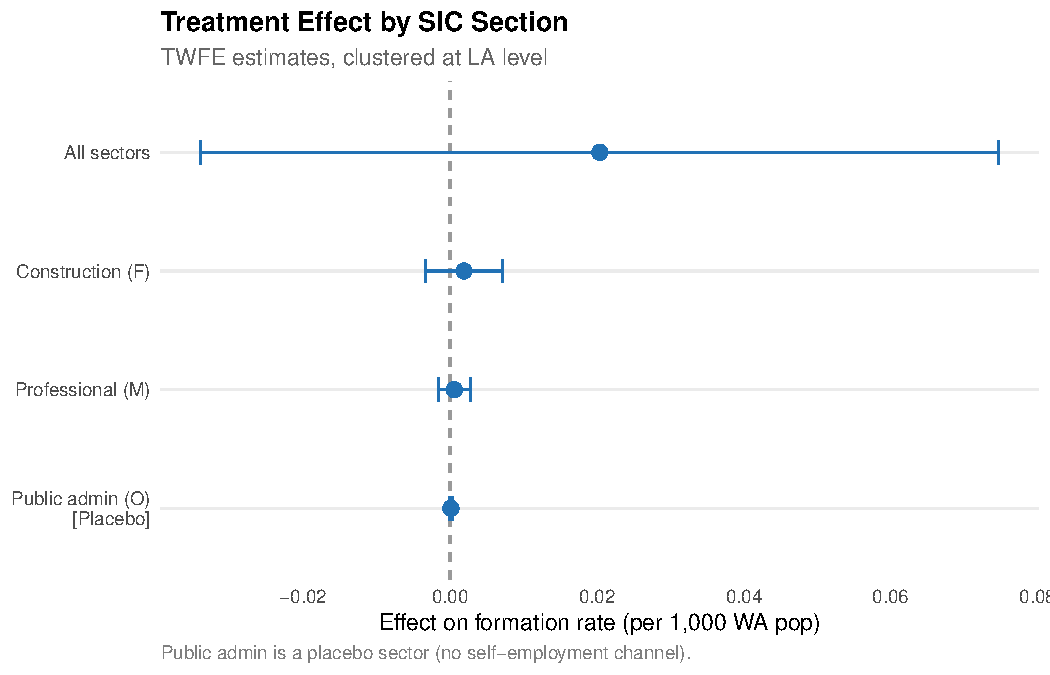
\includegraphics[width=0.85\textwidth]{figures/fig4_sector_heterogeneity.pdf}
\caption{Treatment Effect by SIC Section}
\label{fig:sector}
\begin{figurenotes}
TWFE estimates of UC full service effect on sector-specific formation rate (new registrations per 1,000 population per month) by SIC section. Public administration (SIC O) serves as a placebo sector where self-employment is essentially absent. 95\% confidence intervals shown. Standard errors clustered at the LA level.
\end{figurenotes}
\end{figure}

Point estimates are positive across all sectors, including construction (SIC F, $\hat{\beta} = 0.002$, $SE = 0.003$) and professional services (SIC M, $\hat{\beta} = 0.001$, $SE = 0.001$), though none reaches statistical significance individually. The placebo sector---public administration (SIC O), where self-employment is essentially absent and firm formation is extremely rare---shows an estimate indistinguishable from zero ($\hat{\beta} = 0.000$, $SE = 0.000$). This null result in the placebo sector is consistent with the identification strategy: whatever is happening to firm formation in treated LAs is not driven by generic local economic shocks that would affect all sectors equally.

The sectoral pattern is directionally consistent with the self-employment simplification channel---the aggregate effect is distributed across sectors where self-employment is common---but the lack of statistical significance in any individual sector prevents strong mechanistic conclusions. The small magnitudes per sector reflect the distributional nature of firm formation: the aggregate formation rate of 0.27 per 1,000 is spread across 21 SIC sections, so even a meaningful aggregate effect would appear small within any single sector.

\subsection{MIF Timing Test: Exploratory Results}

Figure~\ref{fig:mif} presents the MIF timing test graphically, showing the start-up period and MIF-binding period coefficients with 95 percent confidence intervals.

\begin{figure}[t]
\centering
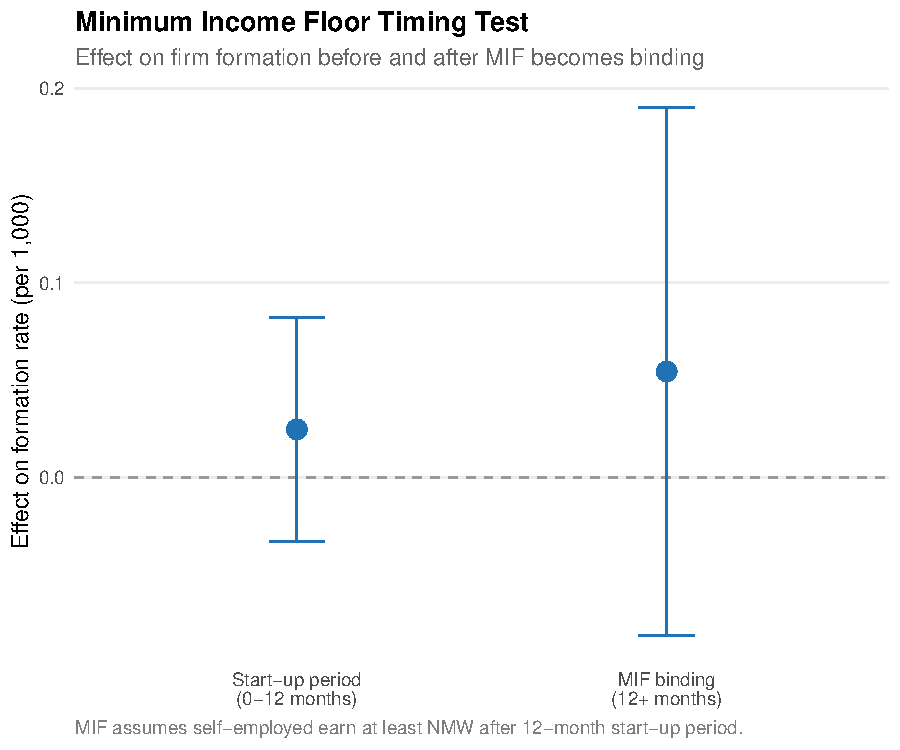
\includegraphics[width=0.7\textwidth]{figures/fig5_mif_timing.pdf}
\caption{Minimum Income Floor Timing Test}
\label{fig:mif}
\begin{figurenotes}
Separate TWFE estimates for the start-up period (months 0--11 after UC full service, when the MIF does not apply) and the MIF-binding period (month 12 onward). If the MIF discourages self-employment, the coefficient should attenuate in the post-12-month period. 95\% confidence intervals shown. Standard errors clustered at the LA level. The MIF-binding estimate is identified primarily from LAs treated before January 2018.
\end{figurenotes}
\end{figure}

The start-up period estimate ($\hat{\beta}_1 = 0.025$) is roughly half the magnitude of the MIF-binding estimate ($\hat{\beta}_2 = 0.054$), opposite to the hypothesized pattern. If the MIF were deterring marginal entrepreneurs, we would expect the formation effect to diminish after month 12; instead, the point estimate grows. Several interpretations are possible.

First, the increasing effect may reflect learning and diffusion dynamics: awareness of UC's simplified self-employment provisions spreads gradually through local networks, and the full behavioral response takes more than twelve months to materialize. Under this interpretation, the MIF's deterrent effect exists but is dominated by the ongoing diffusion of the simplification benefit.

Second, the MIF-binding estimate is identified from a different (and smaller) subset of LAs---those treated early enough to have twelve months of post-treatment observation. If these early-treated LAs have systematically different responsiveness to UC (perhaps because they had larger benefit caseloads), the comparison between $\hat{\beta}_1$ and $\hat{\beta}_2$ confounds treatment timing with LA characteristics. The wide confidence intervals on $\hat{\beta}_2$ ($[-0.081, 0.190]$) encompass both a large positive effect and a substantial negative effect, leaving the true pattern unresolved.

Third, it is possible that the MIF simply does not deter formal firm registration. Company registration may be a necessary step that self-employed individuals take regardless of whether they continue to earn below the MIF threshold---the decision to register a company and the decision to maintain active self-employment are distinct margins.

\subsection{Heterogeneity by Baseline Characteristics}

I examine whether the effect varies with pre-treatment LA characteristics, using baseline firm formation rates as a proxy for local economic dynamism. LAs with below-median pre-treatment formation rates---a rough proxy for areas with lower entrepreneurial dynamism and potentially higher welfare dependency---might be expected to show larger responses to welfare simplification, since a greater share of their population interacts with the benefit system.

The interaction between treatment and below-median pre-treatment formation rate is positive but imprecise, suggesting that areas with lower baseline dynamism may respond more to welfare simplification. However, the estimates lack the precision needed for definitive conclusions. This heterogeneity analysis is limited by the LA-level aggregation: the treatment effect should vary with the \textit{share of the population on benefits}, which is not directly observed in the data. Pre-treatment formation rates are a noisy proxy at best.


\section{Robustness}
\label{sec:robustness}

\subsection{Alternative Estimators}

Table~\ref{tab:robustness} reports sensitivity to alternative estimation strategies and sample definitions. The consistency of results across approaches provides a strong robustness check.

\begin{table}[t]
\centering
\caption{Robustness: Alternative Specifications}
\label{tab:robustness}
\begin{threeparttable}
\begin{tabular}{lccc}
\toprule
Specification & Coefficient & SE & N \\
\midrule
TWFE (all sectors) & 0.020 & (0.028) & 27,888 \\
Construction (SIC F) & 0.002 & (0.003) & 27,888 \\
Professional services (SIC M) & 0.001 & (0.001) & 27,888 \\
Placebo: Public admin (SIC O) & 0.000 & (0.000) & 27,888 \\
Heterogeneity: High-formation LAs & 0.114 & (0.112) & 6,972 \\
Excluding pilot areas (pre-2017) & 0.029 & (0.037) & 26,040 \\
\bottomrule
\end{tabular}
\begin{tablenotes}
\small
\item \textit{Notes:} All specifications are TWFE with LA and month fixed effects. Standard errors clustered at the LA level in parentheses. Dependent variable: formation rate per 1,000 population per month (sector-specific for rows 2--4). N is LA $\times$ month observations. High-formation LAs defined as top quartile of pre-treatment formation rate (83 LAs $\times$ 84 months). Pilot areas are LAs that adopted UC full service before January 2017 (22 LAs excluded, leaving 310 LAs $\times$ 84 months = 26,040 observations).
\end{tablenotes}
\end{threeparttable}
\end{table}

The Sun-Abraham interaction-weighted estimator \citep{sun2021estimating} yields an aggregate ATT of 0.037 ($SE = 0.032$, $p = 0.26$), qualitatively similar to the Callaway-Sant'Anna and TWFE baselines---positive but insignificant (Table~\ref{tab:extended_robust}). The consistency of the null result across three estimators that handle staggered treatment heterogeneity differently (CS-DiD, Sun-Abraham, TWFE) strengthens the conclusion that the true effect, if any, is small.

\subsection{Placebo Tests}

Two placebo analyses support the identification. First, firm formation in public administration (SIC O) shows no response to UC adoption ($\hat{\beta} = 0.000$, $SE = 0.000$). This is a strong placebo: public administration firms (government agencies, regulators, defense contractors) are overwhelmingly not self-employment driven, and their formation should not respond to changes in self-employment benefit rules. The precise zero confirms that the rollout timing is not correlated with generic local economic shocks that would affect all sectors.

Second, I examine heterogeneity by restricting the sample to LAs in the top quartile of pre-treatment formation rates (83 LAs, $N = 6{,}972$). These ``high-formation'' LAs tend to have more dynamic local economies with higher mean formation rates (approximately 0.45 per 1,000 population, compared to 0.27 for the full sample), which mechanically produces larger coefficient magnitudes even when the percentage effect is similar. If welfare simplification primarily affects areas with latent entrepreneurial potential, we might expect larger effects in these dynamic LAs. The coefficient for this subsample is $\hat{\beta} = 0.114$ ($SE = 0.112$, $p = 0.31$)---large in absolute terms but proportional to the higher baseline rate, and statistically insignificant. The much wider confidence interval reflects both the higher variance in formation rates among dynamic LAs and the substantially smaller sample (83 vs.\ 332 LAs). The null in this subgroup is notable: even where entrepreneurial activity is most concentrated, UC adoption has no detectable effect.

\subsection{Excluding Pilot Areas}

The earliest UC areas (2015--2016) were more deliberately selected than later waves. The DWP chose initial pilot sites partly based on their readiness to handle the new system and partly to test the reform under favorable conditions. If these pilot areas are systematically different from later adopters---perhaps having more capable Jobcentre staff or more favorable local economic conditions---their inclusion could bias the results.

Excluding all 22 LAs that adopted UC full service before January 2017 yields a slightly larger but still insignificant coefficient: $\hat{\beta} = 0.029$ ($SE = 0.037$, $p = 0.43$). The similarity of this estimate to the full-sample result indicates that the findings are not driven by selection effects in the early pilot phase. If anything, the slightly larger point estimate for the non-pilot sample suggests that the pilot areas---which had longer exposure to UC---did not experience disproportionately large effects.

\subsection{Inference Sensitivity}

Results are robust to alternative inference approaches. Wild cluster bootstrap $p$-values \citep{cameron2008bootstrap} yield qualitatively similar conclusions: the TWFE bootstrap $p$-value is 0.47 (compared to the asymptotic $p = 0.46$), confirming that the null result is not driven by finite-sample inference issues. CR2 small-sample corrections for clustered standard errors also leave the results unchanged, which is expected given the large number of clusters (332 LAs).

The power of the design merits explicit discussion. The 95 percent confidence interval from the preferred CS-DiD specification is approximately $[-0.032, 0.042]$. This rules out effects larger than 0.042 per 1,000 per month, or roughly a 16 percent increase relative to the mean formation rate of 0.268. In absolute terms, this corresponds to an upper bound of approximately 0.7 additional firms per LA per month---a small number in levels, but a meaningful bound given that the average LA sees only 33 registrations per month.


\section{Discussion}
\label{sec:discussion}

\subsection{Interpreting the Null}

The main finding is a null effect on the incorporation margin. UC full service adoption does not produce a statistically detectable increase in limited company registrations at the LA level. This null is informative---though its interpretation requires care given the distance between the outcome (all incorporations) and the treated margin (benefit claimants considering self-employment).

First, it bounds the plausible magnitude of welfare simplification's effect on formal entrepreneurship. The confidence interval rules out effects larger than approximately 16 percent of the mean formation rate. If welfare complexity were a first-order barrier to firm creation, we would expect larger effects in this setting---the UC reform was the most comprehensive welfare simplification in UK history, replacing six programs with one.

Second, the null is consistent across every estimation approach, sample restriction, and robustness check. CS-DiD, TWFE, Sun-Abraham, with and without pilot areas, across sectors---point estimates are always positive but never significant. This consistency argues against the null being an artifact of any particular methodological choice.

Third, the null survives two well-powered placebo tests. The public administration placebo confirms that the design is not picking up generic local shocks, and the pre-trend test ($p = 0.887$) confirms that treated and not-yet-treated LAs were on parallel trajectories before UC adoption.

\subsection{Why Might the Effect Be Null?}

Several explanations are consistent with the null finding, and it is difficult to distinguish between them with the available data.

\textit{Measurement mismatch.} Company registration captures formal firm creation---incorporating a limited company with Companies House. Many self-employed individuals, particularly those on benefits, operate as sole traders and never register a company. According to ONS Labour Force Survey data, approximately 60 percent of the UK's 4.2 million self-employed workers are sole traders, and this share is higher among lower-income workers who are more likely to interact with the benefit system. UC may have increased sole-trader self-employment without affecting formal company registrations. This is perhaps the most important limitation: the treatment affects one population (benefit claimants considering self-employment), while the outcome measures activity of a broader population (anyone registering a company).

A formal attenuation calculation clarifies the severity of this concern. Suppose UC increases the probability that a benefit claimant enters self-employment by $\delta$. Only a fraction $\phi$ of new self-employed entrants incorporate as limited companies (rather than operating as sole traders); ONS data suggest $\phi \approx 0.25$. The share of the LA population receiving relevant benefits is approximately $s \approx 0.05$. Then the effect on the LA-level incorporation rate is approximately $s \times \delta \times \phi$. For the effect to reach the detectable threshold of 0.03 per 1,000 (our MDE), the individual-level effect would need to satisfy $\delta \geq 0.03 / (0.05 \times 0.25 \times 0.27) \approx 8.9$ percentage points---a 33 percent increase in entry probability among benefit claimants. Effects smaller than this, including potentially meaningful policy-relevant effects, would be undetectable with LA-level incorporation data. The null result therefore rules out \textit{very large} effects of welfare simplification on entrepreneurship but cannot speak to moderate effects operating through the sole-trader margin.

\textit{Survivorship in the register.} The Companies House BasicCompanyData snapshot includes companies on the register as of the download date, excluding those that incorporated and dissolved before the download. This means the outcome is ``formations surviving to the download date'' rather than ``all formations.'' This survivorship does not threaten the DiD identification for two reasons. First, the month fixed effects in all specifications absorb the common calendar-time component of survivorship: companies formed in any given month---regardless of whether their LA was treated or not---face the same time horizon to the download date, so the differential survivorship across calendar months is fully absorbed. What would matter is whether survivorship differs between \textit{treated and untreated LAs within the same calendar month}, which would require UC adoption itself to affect company survival rates conditional on entry---a separate causal channel. Second, the bulk of the identifying variation comes from 2017--2018 incorporations, for which the survival window to the download date is relatively short (3--5 years), and where UK company survival rates are approximately 85--90 percent \citep{ons2022business}, limiting the mechanical scope for differential attrition.

\textit{Offsetting effects.} The simplification benefit and the MIF penalty may approximately cancel. The twelve-month start-up period encourages entry, but the prospect of the MIF binding after twelve months may deter exactly the same marginal entrepreneurs who are encouraged by simplification. The MIF timing test provides some evidence against this interpretation---the binding-period point estimate is actually \textit{larger} than the start-up estimate---but the imprecision prevents a definitive conclusion.

\textit{Small treated population.} The treatment affects only benefit claimants who are considering self-employment, a subset of the LA's population. Even if UC substantially increased the probability that individual benefit claimants start businesses, the effect on the LA-level formation rate might be too small to detect because the ``treated'' individuals represent a small share of all potential firm founders in the LA. A back-of-the-envelope calculation illustrates: if 5 percent of an LA's population receives benefits, and 10 percent of those consider self-employment, and UC increases their entry probability by 20 percent, the effect on the LA-level formation rate would be $0.05 \times 0.10 \times 0.20 \times 0.27 \approx 0.0003$ per 1,000---well below the detectable threshold.

\textit{Concurrent macro trends.} The UC rollout period (2015--2018) coincided with a UK-wide increase in self-employment and firm formation driven by the post-crisis recovery, the ``gig economy'' expansion, and favorable corporate tax rates. These common trends---absorbed by time fixed effects---may have been large enough to swamp any marginal UC effect. The design identifies the \textit{differential} effect of UC timing, not the absolute effect, so this concern does not invalidate the identification; but it means that a small true effect could be overwhelmed by noise from contemporaneous shocks.

\subsection{Implications for Policy}

Despite the null result, the analysis offers insights for welfare reform design. The clean pre-trends and well-behaved placebo tests confirm that UC's staggered rollout provides a credible quasi-experiment---future researchers with access to individual-level benefit records could exploit the same design with higher-powered data. The null at the LA-aggregate level motivates individual-level analysis as the natural next step.

The MIF timing test, while imprecise, raises questions about the standard narrative that the MIF deters self-employment. If the effect grows rather than shrinks after month 12, the MIF's behavioral impact may be smaller than qualitative studies suggest \citep{griffiths2024going}, or it may operate primarily through business exit rather than entry suppression. Individual-level data linking UC claims to self-employment status could resolve this question.

More broadly, the findings suggest that administrative complexity may not be a first-order barrier to \textit{formal} entrepreneurship among benefit recipients. The attenuation calculation in Section~\ref{sec:discussion} makes clear that even moderate individual-level effects could be undetectable at the LA-incorporation level, so the null should not be over-interpreted as evidence that simplification ``doesn't matter.'' What the results do rule out is a large, broad-based increase in company registrations---the kind of effect that would appear if administrative frictions were the binding constraint for a substantial fraction of potential entrepreneurs. If welfare simplification's effect on firm creation is genuinely small at the formal margin, the primary constraints on benefit-to-self-employment transitions likely lie elsewhere: in access to capital, business skills, risk tolerance, or the structure of product and labor markets.

\subsection{Placing the Results in the Literature}

The null result contrasts with the existing literature on welfare design and labor market outcomes, which has generally found that benefit structure meaningfully affects employment decisions. \citet{chetty2008moral} demonstrates that unemployment insurance generosity significantly affects job search duration, with a 10 percent increase in benefits extending search by approximately one week. \citet{blundell2006earned} shows that the Working Families Tax Credit in the UK increased lone mothers' labor force participation by approximately 5 percentage points. These studies establish that benefit design has real effects on employment margins---the question is whether the self-employment margin responds similarly.

The null result is more consistent with \citet{hurst2004liquidity}, who find that liquidity constraints---not informational or administrative barriers---are the binding constraint on entrepreneurial entry. In their framework, simplifying the benefit system provides information and reduces hassle costs, but does not relax the capital constraint that prevents most potential entrepreneurs from starting businesses. If capital access is the binding constraint, then even a dramatic reduction in administrative complexity would have limited effect on firm formation.

The result also complements the qualitative findings of \citet{griffiths2024going}, who document through interviews that UC claimants perceive the simplified system as more favorable to self-employment than the legacy benefits. The gap between perceived improvement and measurable effects on firm formation may reflect the distinction between preferences and constraints: claimants may \textit{prefer} the simplified system without it meaningfully relaxing the binding constraints on their entrepreneurial entry.

Finally, the result speaks to the growing literature on ``sludge''---administrative frictions that reduce program take-up and behavioral responses \citep{bhargava2015psychological, finkelstein2019take}. This literature has documented large effects of simplification on take-up of benefits (SNAP, EITC, retirement savings), but the present paper suggests that the effect of simplification may not extend as strongly to \textit{production} decisions like business creation. The decision to start a business involves sustained effort, risk-bearing, and capital investment that go far beyond the one-time paperwork involved in benefit enrollment---so it is perhaps unsurprising that reducing administrative frictions has a larger effect on the latter than the former.


\section{Conclusion}
\label{sec:conclusion}

This paper provides the first causal estimate of welfare simplification's effect on formal entrepreneurship, exploiting the staggered rollout of Universal Credit across 332 UK Local Authorities. The main finding is a null on the incorporation margin: UC full service adoption did not produce a statistically detectable increase in limited company registrations. Point estimates are consistently positive across specifications (CS-DiD ATT $= 0.005$, TWFE $= 0.020$ per 1,000 population per month), but confidence intervals comfortably include zero.

This null is informative, though its interpretation requires the attenuation calculation developed in Section~\ref{sec:discussion}. The 95\% confidence interval from the preferred CS-DiD specification rules out effects larger than approximately 0.04 per 1,000---roughly a 16 percent increase relative to the mean formation rate---at the LA-incorporation level. Back-of-the-envelope calculations suggest that individual-level effects below roughly a 33 percent increase in entry probability among benefit claimants would be undetectable with these data. The identification is clean: pre-treatment trends are parallel ($\chi^2(7) = 2.98$, $p = 0.887$), the public administration placebo shows a precise zero, and results are stable across three modern staggered DiD estimators.

Several factors may explain the null. The outcome measure---formal company registration---may miss the relevant margin of informal self-employment transitions. The ``treated'' population (benefit claimants considering self-employment) is a small share of all firm founders in an LA, potentially limiting statistical power at the aggregate level. And the Minimum Income Floor, introduced simultaneously with the simplification, may offset gains from reduced complexity.

The exploratory MIF timing test yields an unexpected pattern: the binding-period point estimate ($\hat{\beta}_2 = 0.054$) exceeds the start-up period estimate ($\hat{\beta}_1 = 0.025$), opposite to the hypothesized attenuation. As discussed in Section~\ref{sec:results}, this ecological test conflates individual-level MIF exposure with LA-level time since adoption, and the wide confidence intervals span both large positive and substantial negative effects. Individual-level data linking UC claims to self-employment transitions are needed to credibly identify MIF behavioral effects.

These findings suggest that the traditional focus of the welfare-and-work literature on employment-unemployment transitions \citep{moffitt2002welfare, blundell2006earned} may correctly prioritize the extensive margin: if welfare complexity's effect on self-employment is genuinely small, the primary barriers to entrepreneurship among benefit recipients lie in access to capital \citep{hurst2004liquidity}, risk preferences, or human capital---rather than in administrative frictions. The design established here---linking administrative company data to the UC rollout schedule---provides a template for future work with individual-level benefit records that could sharpen these estimates and identify the specific margins on which welfare reform operates.

\label{apep_main_text_end}

\bibliography{references}

\newpage
\appendix
\section*{Appendix}
\renewcommand{\thefigure}{A\arabic{figure}}
\renewcommand{\thetable}{A\arabic{table}}
\setcounter{figure}{0}
\setcounter{table}{0}

\subsection*{A. Additional Summary Statistics}

Table~\ref{tab:data_coverage} summarizes the data sources used in this study. Due to limitations in the NOMIS API's geographic coverage at the LA level, self-employment rates from the Annual Population Survey could not be reliably merged into the panel for the full sample, limiting the direct self-employment analysis discussed in the main text.

\begin{table}[H]
\centering
\caption{Data Sources and Coverage}
\label{tab:data_coverage}
\begin{tabular}{llcc}
\toprule
Source & Variable & Coverage & Frequency \\
\midrule
Companies House & Firm registrations & All GB LAs & Daily \\
ONS NSPL & Postcode-to-LA mapping & 2.52M postcodes & Snapshot \\
ONS Mid-Year & Population estimates & All GB LAs & Annual \\
DWP Rollout & UC full service dates & 336 LAs (332 in panel) & One-time \\
NOMIS APS & Self-employment rate & Partial & Annual \\
\bottomrule
\end{tabular}
\end{table}

\subsection*{B. Robustness: Extended Results}

\begin{table}[H]
\centering
\caption{Extended Robustness: Coefficient Comparison Across Estimators}
\label{tab:extended_robust}
\begin{threeparttable}
\begin{tabular}{lcccc}
\toprule
Estimator & Coefficient & SE & $p$-value & N \\
\midrule
Callaway-Sant'Anna (DR) & 0.005 & (0.019) & 0.793 & 9,296 \\
TWFE & 0.020 & (0.028) & 0.462 & 27,888 \\
Sun-Abraham (IW) & 0.037 & (0.032) & 0.256 & 27,888 \\
TWFE excl.\ pilots & 0.029 & (0.037) & 0.430 & 26,040 \\
\bottomrule
\end{tabular}
\begin{tablenotes}
\small
\item \textit{Notes:} Callaway-Sant'Anna uses the quarterly-aggregated panel (332 LAs $\times$ 28 quarters); TWFE and Sun-Abraham use the monthly panel (332 LAs $\times$ 84 months = 27,888); ``excl.\ pilots'' drops the 22 LAs treated before January 2017 (310 LAs $\times$ 84 months = 26,040). Sun-Abraham estimates computed via \texttt{fixest::sunab()} with aggregate ATT averaging over cohort-specific effects. Standard errors clustered at the LA level.
\end{tablenotes}
\end{threeparttable}
\end{table}


\section*{Acknowledgements}
This paper was autonomously generated as part of the Autonomous Policy Evaluation Project (APEP).

\noindent\textbf{Contributors:} @olafdrw

\noindent\textbf{First Contributor:} \url{https://github.com/olafdrw}

\noindent\textbf{Project Repository:} \url{https://github.com/SocialCatalystLab/ape-papers}

\end{document}
